\documentclass[12pt]{article}
\usepackage[a4paper, total={6in, 8in}]{geometry}
\usepackage{tikz}

\begin{document}
	\section*{Testbeispiele}

	\begin{figure}[!ht]
		\begin{center}
		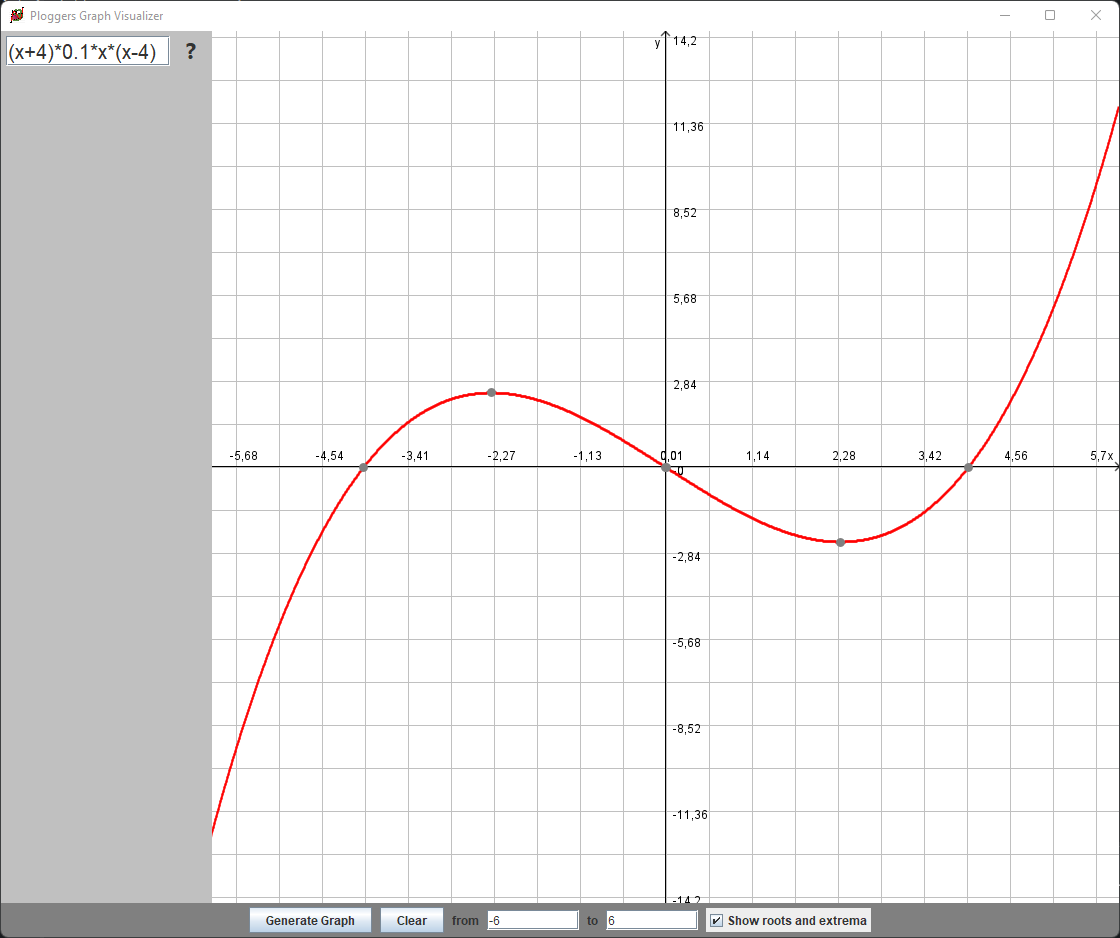
\includegraphics[scale=0.75]{images/sample1.png}
		\end{center}
		\caption{Polynom - $f(x) = (x+1.5)(x-1.5)x$}
		
		\begin{center}
			\texttt{(x+1.5)*x*(x-1.5)}
		\end{center}
	\end{figure}

	\begin{figure}[!ht]
		\begin{center}
		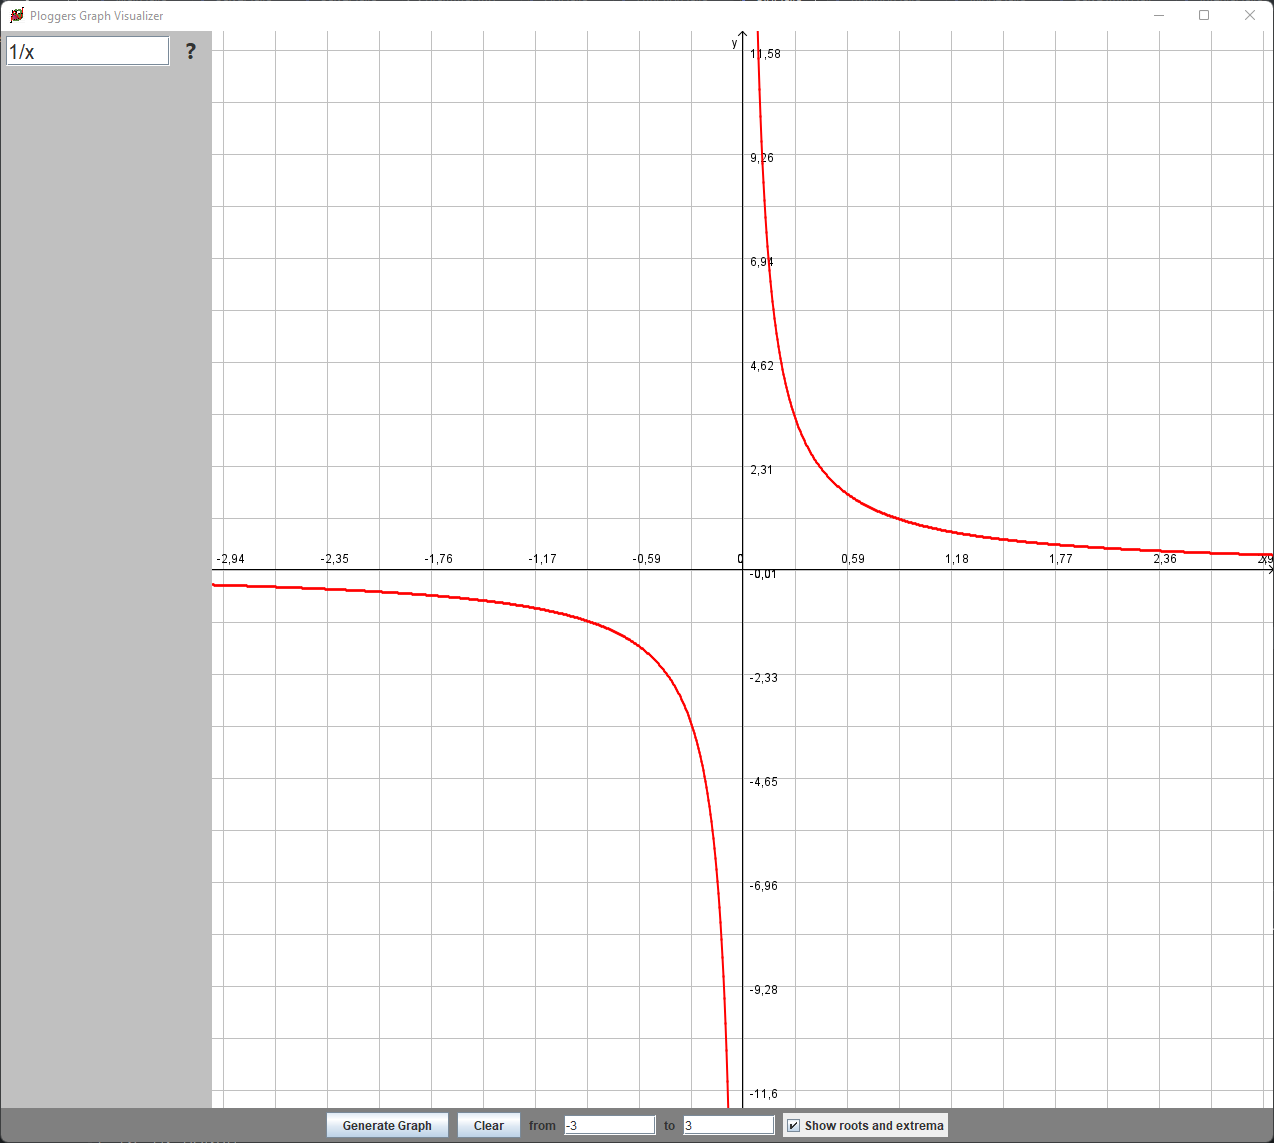
\includegraphics[scale=0.75]{images/sample2.png}
		\end{center}
		\caption{$f(x) = \frac{1}{x}$}

		\begin{center}
			\texttt{Hyperbel - 1/x}
		\end{center}
	\end{figure}

	\begin{figure}[!ht]
		\begin{center}
		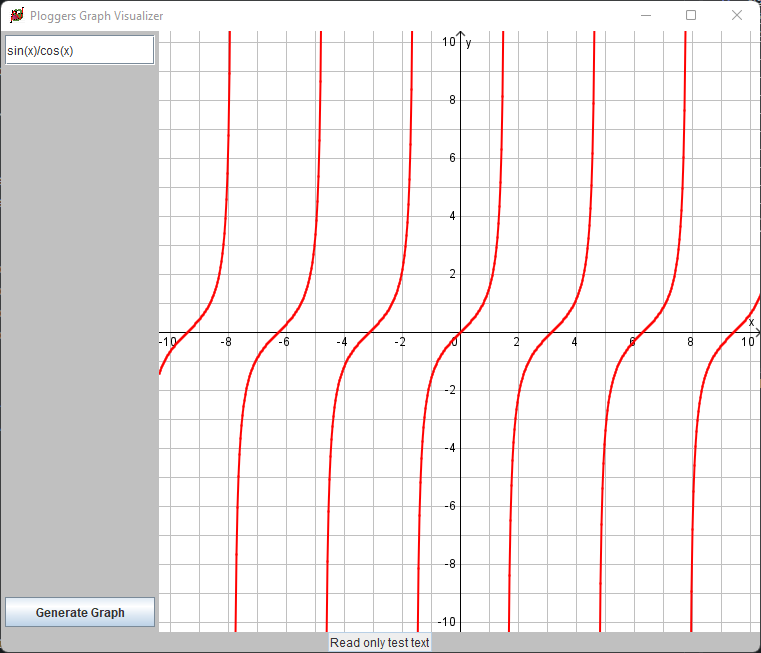
\includegraphics[scale=0.75]{images/sample3.png}
		\end{center}
		\caption{$f(x) = \frac{\sin{x}}{\cos{x}}$}

		\begin{center}
			\texttt{Tangens - sin(x)/cos(x)}
		\end{center}
	\end{figure}

	\begin{figure}[!ht]
		\begin{center}
		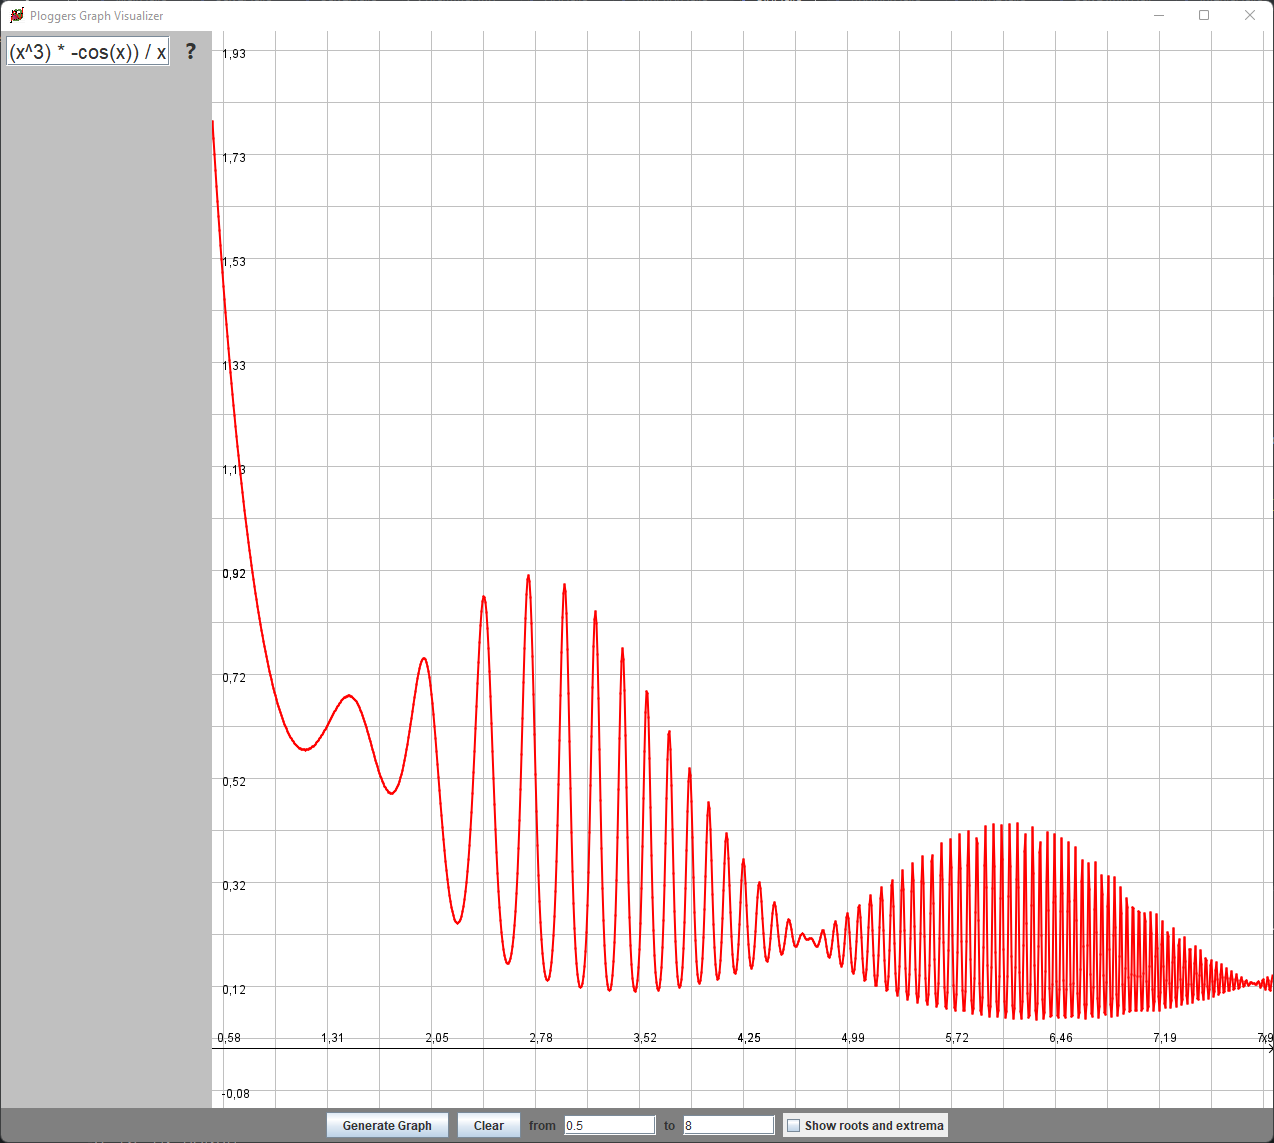
\includegraphics[scale=0.5]{images/sample4.png}
		\end{center}
		\caption{$f(x) = \frac{\exp(\sin{x^3} * -\cos{x})}{x}$}

		\begin{center}
			\texttt{Kompliziert - exp(sin(x\textasciicircum 3) * -cos(x)) / x}
		\end{center}
	\end{figure}

	\begin{figure}[!ht]
		\begin{center}
		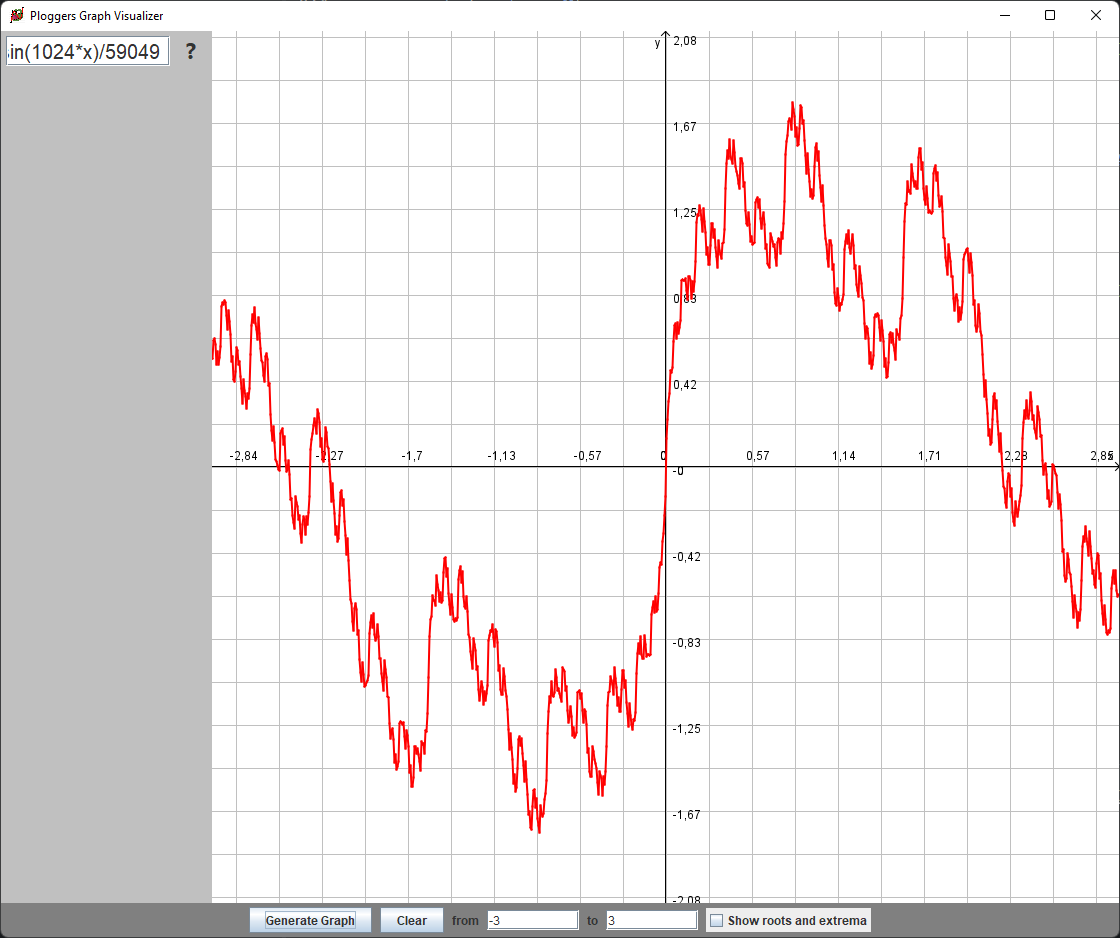
\includegraphics[scale=0.65]{images/sample5.png}
		\end{center}
		\caption{Weierstraß - $f(x) = \sum_{k=0}^{10} \frac{2^k \sin(2^k x)}{3^k}$}

		\begin{center}
			\texttt{sin(x) + 2*sin(2*x)/3 + 4*sin(4*x)/9 + 8*sin(8*x)/27 + 16*sin(16*x)/81 + 32*sin(32*x)/243 + 64*sin(64*x)/729 + 128*sin(128*x)/2187 + 256*sin(256*x)/6561 + 512*sin(512*x)/19683 + 1024*sin(1024*x)/59049}
		\end{center}
	\end{figure}
\end{document}